% $Id: $
\documentclass[a4paper,12pt]{report}

% The following makes latex use nicer postscript fonts.
\usepackage{times}
\usepackage[english]{babel}
\usepackage[colorlinks,urlcolor=blue,linkcolor=blue]{hyperref}
\usepackage{wrapfig}

\usepackage{vubtitlepage}
\author{Ayrton Vercruysse}
\title{TIAMAT: A Multi-touch Tablet IDE for AmbientTalk}

%\promotortitle{Promotor/Promotors}
\promotor{Prof. Dr. Wolfgang De Meuter}
\advisors{Dries Harnie\\
          Lode Hoste}
\faculty{Faculty of Science}
\advisortitle{Advisors}
\department{Department of Computer Science\\ and Applied Computer Science}
\reason{}

\date{2012-2013}
          
\begin{document}

\maketitlepage
\tableofcontents
\chapter{Introduction}
\section{Goal}



\section{Scope}
The scope of this project is a third bachelor thesis at the Vrije Universiteit Brussel. The 3th bachelor thesis is given at third bachelor students computer sciences. The goal of this bachelor thesis
is to let the bachelor students  participate in some actual research at the university. This has been chosen over giving the students a predefined task.
\section{Definitions and Acronyms}

\begin{tabular}{ l l }
  VUB & Vrije Universiteit Brussel \\
  IDE & Integreted Develepment Environment \\
  AST & Abstract Syntax Tree \\
  MANET 	& Mobile Ad-Hoc Network \\
  OHA & Open Handset Alliance \\
  App & Application. Programs on smart phones and tablets \\
  MT4j & Multi-Touch for Java \\
\end{tabular}
\chapter{Implementation}
\section{Used Software}
\subsection{AmbientTalk}
AmbientTalk is a programming language developed at the VUB in 2005. The goal of the language was to focus on making programs within Ad-Hoc networks. This means that AmbientTalk is developed mainly
to create programs on mobile devices. AmbientTalk combines elements from other programming languages such like Scheme (closures), Smalltalk (pure OO), Self (prototypes and delegation) and some
other languages.

AmbientTalk was originally a part of a doctorate study made by Jessie Dedecker. His goal was to create an extension to the already existing programming language Pic\% (pic-oh-oh). Pic\% itself
was an extension of Pico. Pico was developed by professor Theo D'Hondt in 1996. Pico was developed merely to be used with an educational purposes. Pico is being used as a programming language to
illustrate how programming languages are being made.

Pico got it's design principles and concepts from Scheme. The goal of Pico was to be a programming language based on simple rules, easy to extend. Thanks to the simplicity and extendability of Pico
this language is often used to do some research to possible extensions and features for programming languages. This is the reason why a lot of offsprings of Pico are created, all with their own
special attention to certain problems or extensions. When AmbientTalk was being developed special attention was given create distributed programs within ad-hoc networks.
Momentarily AmbientTalk/2 is being used. It's the successor of the original AmbientTalk. Even though AmbientTalk/1 was already successful concerning the programming features for mobile Ad-Hoc
networks it lacked some important features to create bigger software applications, such like exception handling,...

In 2006 Tom Van Cutsem and Stijn Mostinckx started developing AmbientTalk/2, the current version of AmbientTalk. The changes between AbmientTalk/1 and AbmientTalk/2 are quite big. There has been
made an entire new design for most aspects of the language, including the syntax. The reason to change the syntax was to make AmbientTalk more accessible for people who don't have any experience
with Pico. 

AmbientTalk is still mainly used by students at the VUB to do some research. But, slowly but surely, AmbientTalk became a useful, handy programming language which was usable to create some
rather big programs. Because the focus of AmbientTalk lies within the distributed networks and this is still an area in which a lot of research is being done there aren't a lot of good alternatives.
This made AmbientTalk a good alternative to create some real-life software.

The symbiosis with the underlying Java Virtual Machine enables the possibility to use some parts of the Java programming languages within AmbientTalk, which makes it possible to combine both languages within
one project.

The renewing element of AmbientTalk is so big that it became the main subject of the Distributed and Mobile Programming Paradigms course taught at the VUB.
\subsection{Google Android}



\subsubsection{General}
\begin{wrapfigure}{r}{0.5\textwidth}
  \begin{center}
    
\includegraphics[width=0.48\textwidth]{images/android.png}
  \end{center}
  \caption{Android logo}
\end{wrapfigure}
Android is an open source platform for mobile devices, owned by Google. Android is developed by Android Inc., a company bought by Google in 2005, which later placed it 
within the Open Handset Alliance (OHA). 

It's an on Linux based operating system and is mainly programmed in C (core), Java (UI) and C++.

Android is originally created by Android Inc., a company founded by Andy Rubin, Rich Miner, Nick Sears and Chris White in 2003. Their goal was to create an operating system
for " ... smarter mobile devices that are more aware of its owner's location and preferences.`` 

On October 17th 2005 Google bought Android Inc. and made it a part of their company. Even after Google bought the company founders Andy Rubin, Rich Miner and Chris White
kept working for Android. Already back then the goal of Google was to focus on the market of mobile devices with Android.

Only on December 9th 2009, together with the founding of OHA, the first product of Google concerning the market of the mobile devices was announced; Android. An on Linux 
kernel version 2.6 based platform for mobile devices.

According to estimations in the second quarter of 2009 approximately  2.8\% of new smartphones had Android as operating system. In the fourth quarter of 2010 this number
had grown to 33\% what made it the best selling smartphone platform. In the third quarter of 2011 this would already have grown to 52.5\%. In February 2012 Andy Rubin
said that Google activates 850000 smartphones or tablets on a daily basis. 
\begin{figure}
  \centering
    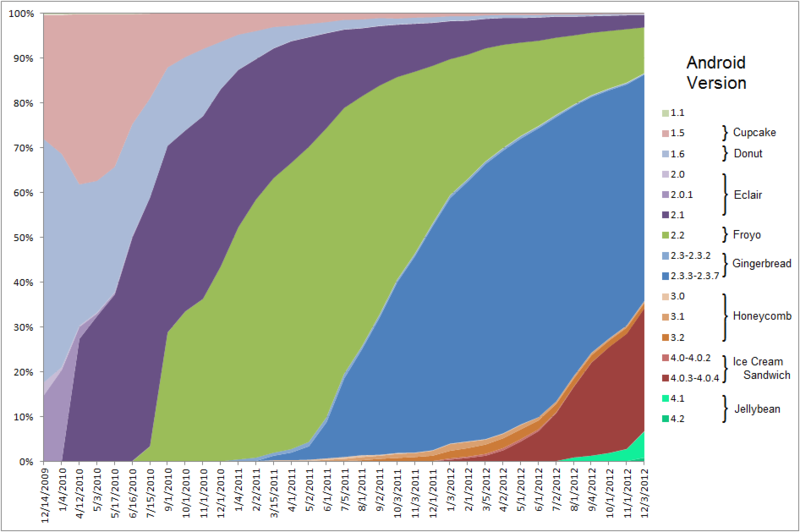
\includegraphics[width=0.99\textwidth]{images/Android_historical_version_distribution.png}
  \caption{Android historical version distribution}
\end{figure}

\subsubsection{Versions}
Through the years multiple versions of Android have been released. In November 2007 a beta version was released, but only on September 23th 2008 Android 1.0 was released.
Android 1.0 was introduced on the HTC Dream. This version was already equipped with the Android Market, an application which gives you the option to download and update
new applications, camera support, synchronization with, and use of, most Google products, like Gmail, Google Calendar, Google Contacts, Google Search, Google Talk,... 
Also Wi-Fi and bluetooth were already supported, just like a Youtube media player.

After Android 1.0 in February 2009 Android 1.1 was released. After Android 1.1 a next version of Android, Android 1.5 which was given the name Cupcake was released followed by 
Android 1.6, called Donut. In October 2009 Android 2.0 got released. It was called Eclair. Eclair was followed by Froyo (2.2.x) and later the popular Gingerbread (2.3.x)
Next to the 2.x series in February 2011 the 3.x (Honeycomb) version got released. This version was created with focus on tablets and no longer on smartphones.

In October 2011 Android 4.0.1 (Ice Cream Sandwich) was presented. ICS was the version of Android which should combine the 2.x series and 3.x series to the 4.x series.
This means that there will be no longer 2 parallel versions of Android, but only one, working on both smartphones and tablets. This made it easier for Google, so they 
didn't need to keep two versions up to date but only one. On July 9th 2012 a new version of the Android 4.x series was released named Jelly Bean (4.1).
In Figure 1.2 one can see a chart showing global Android version distribution from November 2009 to December 2012.

\subsubsection{Design}

Android is based on a Linux kernel, with middleware, libraries and APIs written in C and application software in Java. In Figure 1.3 the architecture of Android is shown.
The top layer of the figure; the Application Layer are the applications which are deployed on the phone when bought, like an SMS program, calendar, internet browser,...
All these applications are written in Java. The application framework is made to create an open developing platform. Android gives developers the possibility to develop
rich and innovative applications, by giving them the liberty to make use of all hardware, like location information, setting alarms, add notifications to the status bar,...

The libraries layer contains a number of C/C++ libraries which are being used in multiple layers of the Android system. Developers are able to explore these libraries
trough the Android Application framework for developers. Some of these libraries are SGL (an underlaying 2D engine), FreeType (a bitmap and vector renderer), MQLite (a 
database engine),... The Android Runtime part is a number of core libraries which gives most Java functionalities. Last there is the Linux kernel which provides safety, memory
management, process management, network stacking and driver models. It also functions as abstraction layer between the hardware and the rest of the software.
\begin{figure}
  \centering
    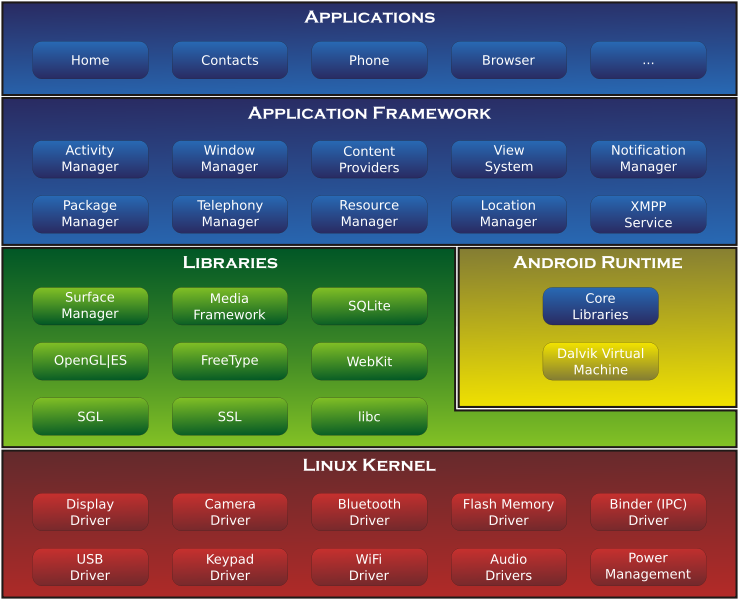
\includegraphics[width=0.99\textwidth]{images/Android-System-Architecture.png}
  \caption{Android System Architecture}
\end{figure}
\subsubsection{Open Handset Alliance}
The Open Handset Alliance (OHA) is a consortium of 84 firms to develop open standards for mobile devices. Practically this translates in promoting Android. OHA is founded
on November 5th 2007, with as main founding company Google, together with 34 other firms. These firms are active in creating software, creating mobile devices or creating
chips. The main goal was to make Android a worthy competitor of other mobile platforms like those developed by Apple, Microsoft, Nokia (Symbian), HP, Research in Motion 
and Barda.

Some of the companies who aided founding OHA were, besides Google, HTC, Sony, Dell, Motorola, Qualcomm, Texas Instruments, Samsung Electronics, LG Electronics, T-Mobile,
Nvidea,... 
\subsection{MT4j}
\subsubsection{General}
Multi-Touch for Java is developed to make it possible to create multi touch applications within the Java programming language. It's an open source Java Framework. It offers a GUI in which we can use
shapes like rectangles, rounded rectangles, ellipses, polygons,... To each of these forms gestures can be attached. These can be in 2D or 3D. Next to the predefined shapes you can also make use 
of buttons, text areas, sliders and a multi touch keyboard.
\subsubsection{Architecture}
The architecture of MT4j is built in multiple layers which communicate with each other. Using event messages which are sent from one layer to another. The different layers within MT4j are the 
Presentation Layer, Input Processing Layer, Input Hardware Abstraction Layer and the Input Hardware Layer.
\begin{figure}
  \centering
    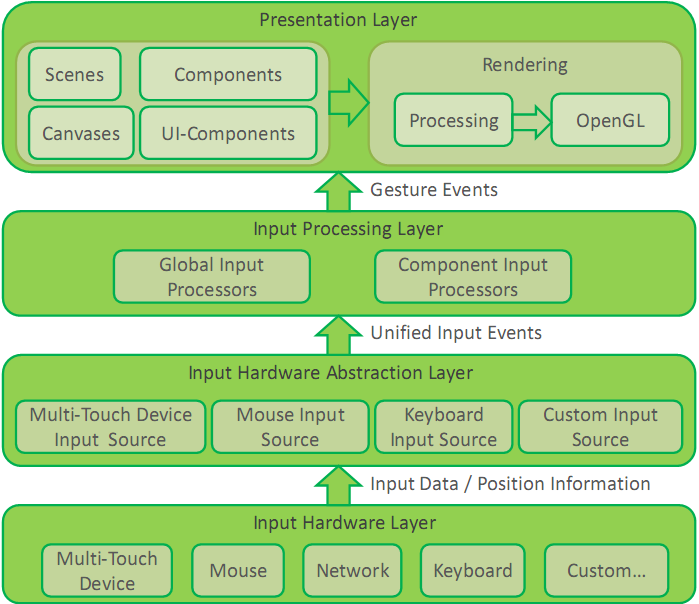
\includegraphics[width=0.99\textwidth]{images/ArchitectureOverview2.png}
  \caption{MT4j Architecture}
\end{figure}
\\
\\
\textbf{Input Hardware Layer}
\\
By making use of the Input Hardware Abstraction Layer MT4j can give support to different kinds of input hardware, while only little alternations are needed within the Hardware Abstraction Layer.
Within this layer all raw input gets reformed to unified input events. The only change needed when one wants to use a new form of input is to change the abstract superclass of all input sources
and the specific input for this new part of hardware.
MT4j already has a number of input methods which are supported, like a keyboard, mouse,... All input methods can be used synchronously and together without chances on conflicts.
\\
\\
\textbf{Input Processing Layer}
\\
In MT4j the input processor gets used on two moments within the input event flow. The first moment is when input directly from the Input Hardware Abstraction Layers comes, the other moment
is at the component level. This means one can recognize gestures which are meant for only one component.
\\
\\
\textbf{Presentation Layer}
\\
The Presentation Layer within MT4j uses scenes. Scenes are made to be able to separate different aspects of a program, input and output, in a nice clean encapsulated 
manner. An example of multiple scenes could be a game where there's one scene to create the menu and an other scene in which the actual game is played.

Next to scenes MT4j also uses components. Components are parts of a program which can be connected in a hierarchical manner. So one can use a basic component and add multiple
components within this component. Here we can see as the basic component the background of the application, and within this component one or more other components are used.

The most basic component of MT4j is a canvas. A canvas is the link between multiple components and the input of the hardware. It can check what other components are on
what place within the screen at a given time.

To render the MT4j components they use the Processing toolkit. Processing is an open source toolkit that is used to create data visualization and interaction.

\subsubsection{MT4Android}
MT4Android is an Android version of MT4j. Because MT4j lays the focus on multi touch and is made within Java it seemed a logical step to port MT4j to the Google Android 
platform. MT4Android is made by a coworker of MT4j. MT4Android still isn't a full version, but there is a beta version available.


\chapter{Implementation Details}
\section{ASTs}
 Every piece of code used in the IDE will be directly linked to an AST. For this matter there has to be a possibility to create new ASTs from scratch.
To create new ASTs we will need to implement the different parts of which an AST can exist. These different parts of an AST will be called a Nodes. We will start with
a list of possible nodes with which basic programs can be made. Later extra kinds of nodes can be added to the AST.

A superclass Node will be implemented which will organize the tree structure by providing operations as follows;
\newline\textbf{getParent()}: gets the parent of a Node, this function is used when we want to replace a node, to do so we replace the child of the parent (this node) to another node.
\newline\textbf{setParent(Node parent} : sets the parent to a new node. This function is used when we want to copy our node to another place, or when a new node is introduced as a child of another node.
\newline\textbf{getChilderen()}:  this functions returns a vector with all child nodes of the node. 
\newline\textbf{getChild(int i)}: returns the i'th child in the children vector of the node. This is often used when we use some tree traversing trough the tree. For example when we call toXML() on a Node we will also 
use a for loop over all of it's children calling the toXML() function.
\newline\textbf{addChild(Node node)}: This function adds a child to the Node. This function is used when we create certain instances of Nodes. By initializations they often add children.
\newline\textbf{setChild(Node oldChild, Node newChild)}: This function replaces an old child node with a new child node. This function is mostly used to replace Placeholder nodes with actual nodes.
\newline\textbf{getNumberofChildren()}: This function return the total number of children, or the length of the children vector. Just like the getChild(int i) operation this function is used to traverse all children of a node
using a for-loop.
\newline\textbf{isRoot()}: This function checks whether this function is the root node. In other words it checks if the parent of the function is null.
\newline\textbf{toString()}: This function translate the node to actual AmbientTalk code. This code is used to write to a textfile, so it can be called in the AT app.
\newline\textbf{toXML()}: This function translates the Node to it's XML representation. This so we can store a node in an XML file.
\newline\textbf{clone()}: This function makes a deep clone of the node, this is done so we can reuse templates, without them having the same parents.
\newline



All kinds of nodes we will use are defined as subclasses of the Node class. The currently implemented sorts of node are:
\newline\textbf{ArgumentList: } An ArgumentList is as the name tells us a list of arguments. This is used in a various other functions.
These can be just a function, or a whenever:discovered: or other functions.
\newline\textbf{Begin: } A begin is used to combine various other parts of code. 
\newline\textbf{Block: } A block is very similar to a argument list, but in stead of using curly braces we use pipes.
\newline\textbf{Definition: } A definition is used to define things like values.
\newline\textbf{Function: } The function node keeps all defined functions. These functions are used in the templates, or after a
function definition to keep functions.
\newline\textbf{FunctionCall: }The function call node is the node used to call a predefined function. Whenever a new function is created with the functionDefinition node we automatically will create
a functionCall node so the function can be called later on.
\newline\textbf{FunctionDefinition: } The FunctionDefinition is used to be able to define new functions.
\newline\textbf{Operation: } An operation are things like +,-,*,/. This node keeps an operator en two placeholders to create the operation.
\newline\textbf{Placeholder: } A placeholder is something we use to say something meaningful needs to come here, but isn't yet. Each placeholder is showed with a red background and can have a specific string as 
text.
\newline\textbf{Table: } This node represents a table. When creating a table you enter the amount of elements you want to insert in the table, and for each of these elements a Placeholder is created. 
\newline\textbf{TableCall: } A tablecall is used to get a certain element from a table. For this an placeholder is created where you enter the element you want to get.
\newline\textbf{TableDefinition: } This is used to create a table. This has a name for the table, a number of elements in the table and a begin in which we can put the way the table has to be created.
\newline\textbf{Value: } A value is just a value, represented as a string. When we create a function and we want to give the function a name this function name is a value, the value of the function name. 

If we take a look at our prestudy document, listing all the requirements we need we can using this implementation a lot of requirements in the ASTs section.
Requirement 2.1.1 Making ASTs can be done, as every node has it's own creation function, Requirement 2.1.2 Deleting ASTs can be accomplished by using the sets provided for the nodes. You can delete a node by
simply replacing it by a Placeholder node. Requirement 2.1.3 Replacing parts of ASTs can be completed in the same way as 2.1.2 by using the setChild and setParent functions.

For Requirement 2.1.4 Rendering ASTs to text we have to toString() function provided in each Node. An extra requirement that could have been added here is Translate AST to XML, for which the toXML() function has been created.


\section{Templates} 
Templates are the connection between the previous defined nodes and the writing of code. Templates are a predefined number of nodes in an order to create some basic code. This means that we have some templates like 
and if-then-else function, which is kept as a function node. Other things that are kept in templates are operations, like the +,-,*,/ operators. To make some useful code we of course make use of things like if-then-else
statements and operation, and we're not planning to create them ourselves. 

All templates that can be used within the the project are predefined in XML. There is an XML file called templates.xml, the reason we chose this is so people can easily add some templates themselves, without having 
to browse trough any code. Most people planning to use the app have a basic knowledge of XML and won't have any problem to add these templates to the file.

All stuff concerning reading templates, writing templates and creating templates are kept in the vub.templates package. Here we have a Templates class, which creates a new template. This in fact does nothing more than adding
a name to a function. Next to these we also have a TemplateReader and a TemplateWriter class.

The templateReader class will, making use of the asset manager read the xml file and then it will loop over all defined templates defined in it. It will check what sort of template it is and then will call the
constructor class of the node of which this template is made. The node will return a new instance of the content of the template and then the template reader will add the newly created node to the right vector that
stores the templates.

In total there are 3 vectors storing templates; functions, like if-then-else or when-discovered, operations, like +,-,*,/ and definitions, like blocks, value's, tables,...

After we've read all the templates and they are added to their vector we can read these vectors and create menu's with these templates as possible building blocks for writing code.

Besides reading templates we also write templates. To write templates we have a toXML() function in each node, so the only thing this class needs to do is write the created XML to a file on the tablet's storage. The templateWriter
can be used to define own functions and keep them as new templates, or to save the current working file and save this, so we can carry on from the saved file later on.

As templates are made to be easily to implement yourselves only a small number of templates are already defined in the system. For functions these are templates like if-then-else, when-discovered, while-do, when-becomes,
whenever-disconnected, whenever-reconnected, and println. For functions these are the basic functions like addition, subtraction, multiplication and devision. In the definitions category we have values, functions, tables, begins,
and blocks. These are off course not more dependable on the existing nodes and are not as easy to add yourselves like the operations and functions are.

If we take a look at the requirements of the project concerning templates we have Requirement 2.2.1 Templates Creating ASTs, this template has been fulfilled because of every node has a creator function using templates.
Requirement 2.2.2 Creating Templates from XML is fulfilled because of the same functions. The last requirement concerning templates, Requirement 2.2.3 Create templates from function is fulfilled because of the toXML() function
written in each subclass of Node. At the moment there is no buttons yet to add a new function from within the app, but this can easily be added.

% \subsection{Templates creating ASTs}
% \textbf{Description: } For convenience we will make use of templates. Templates will be frequently used parts of code that will be saved. The way templates will be stored in the 
% memory will be by an AST. Every time a template is used withing the program a copy of this AST will be made and inserted into our current program.
% These templates can be frequently used functions, but mainly these will be the ASTs representing basic elements of the language like the if-then-else structure, when-discovered,...\newline
% \textbf{Priority:} High \newline
% \textbf{Status: }There is a file called 'templates.xml' containing all templates that we currently use. Within the TemplateReader class these templates are being read and translated to ASTs. \newline
% \subsection{Creating templates from XML}
% \textbf{Description: } To keep a clear view on what template functions we have, and make it easy for users to add templates, without having to know the implementation
% of the entire program we will keep the Templates in a separate XML file. When having an XML file containing the structure to create new Templates a function will be implemented that creates, from the XML file, a new AST, which 
% can be used as a Template within the program.\newline
% \textbf{Priority:} High \newline
% \textbf{Status: }There is a file called 'templates.xml' containing all templates that we currently use. Within the TemplateReader class these templates are being read and translated to ASTs. \newline
% \subsection{Create templates from functions}
% \textbf{Description: } When a newly created function is often used by the user and he wants to save this function, the possibility to write this function, in correct XML, to
% the existing XML file will be provided. This means that whenever the program is terminated functions can be stored inside the XML file.\newline
% \textbf{Priority:} Low \newline
% \textbf{Status: } Every new function that is being created is saved as a template within the program. As every node has the possibility to be translated to XML it is fairly easy to add the option to write this XML to 
% an XML file.\newline
\section{Interface}
\subsection{Rendering of nodes}
Besides having the nodes representing the AST internally we still need a way to show them on the screen. To show nodes on the screen we have everything defined in the vub.rendering package. This package contains a Renderer 
class and subclasses for each type of node. The reason we have created separate classes is to not pinned down to one representation of either the AST or the rendering of the nodes. This means that the AST part of this project
can be reused in other projects, or that we can replace the entire way the AST is printed on the screen within the project, to make it, for example run on a pc.

To keep the connection between the AST and the rendering of the AST we have implemented a visitor class called RenderVisitor. This class makes sure that whenever a Node needs to be rendered that we call the right
rendering class for this particular node. The only thing the rendering classes need to worry about is how to display a certain node to the screen. For an operation like the addition for example this is making an opening and
 closing bracket, making an the operator sign and call the display function of both of the arguments. After this he needs to make sure all of this is shown in the right order and on the right place within the rest of 
the code. 

To handle this we've implemented the RenderManager class, winch is a lay-out engine that manages the places where all separate parts of the code need to be rendered. Thanks to this manager we didn't have to manager 
exact locations within the display function of each node, but we only had to call the lay-out engine saying: render this bit next to the previous code. 

To make reading the code a bit easier we gave particular sorts of nodes special attention. When a node is selected it is surrounded by a red square, so you can easily see with what node you are working on the moment. For Placeholder
nodes we have chosen to turn the back of the placeholder red. Because a Placeholder is in fact not really useful in a program, it is easy when you can see where they are situated so you can change them around quite fast.

Next to this the values are shown in blue. These values can be variables, or the name of a function.

\subsection{Buttons}
Next to the Nodes we need more stuff rendered to the screen. These are things like buttons and menu's so we can interact with the code. For menu's an entire separate package is creates called vub.menus. This package contains a 
base Menu class and some subclasses made for every sort of ASTs, like a definitions menu, a functions menu, an operations menu, a variables menu and a menu for own defined functions. To browse trough all these menu's there is 
a beginMenu what gives you the opportunity to browse between these other menu's.

For each definition of a value or a function a new buttons is added to the menus representing this. If you for example set the value of variable x to 5 by saying def x = 5 then automatically we will add x to
the value menu so you can easily reuse your variable x. The same counts for functions. whenever a new function is made a functionCall node is created and is placed within the MyFunctionsMenu.

Next to the buttons in the menu's 3 other buttons have been created on the screen. These are the save-button the delete-button and the run-button. As you can guess the save button will save the file. It will call the 
toXML() function of the main node and hand this result to the TeplateWriter so it can be written to an XML file.

The delete button is made to delete parts of code. This can be done by dragging code to the bin and dropping it right on it, or selecting a piece of code and then hit the delete button. Every piece of code that gets 
deleted will be replaced by a Placeholder containing the text 'deleted'.

As a last you have the run button which will translate the code to AmbientTalk, using the toText() function of the main node, store it in a file and hand it over to the AmbientTalk interpreter situated in the RunAT class in the 
vub.tiamat package.



% \subsubsection{Menu's}
% \textbf{Description: } To keep track of all templates or calls that can be made we will need a menu that gives us the possibility to insert templates in to the code.
% We will use one a menu with some sub menu's, divided for each kind of templates. These can be provided functions self implemented function, used variables,... \newline
% \textbf{Priority:} High \newline
% \textbf{Status: } In the package vub.menus all menus that are available in the program are implemented. These are a standard menu, a menu for functions, operations, own functions, definitions, variables, ...\newline
% \subsubsection{Run button}
% \textbf{Description: } Thanks to requirements 4.2 we can evaluate made code with an external AmbientTalk app. To do this we'll add a button
% to the main screen which will first make sure requirement 1.4 is done, the creation of a text file with the current code, and later on run the AmbientTalk app, as described in requirement 4.2.
% \textbf{Priority:} High \newline
% \textbf{Status: } The implementation of this button can be found in the Tiamat class within the vub.tiamat package.\newline
% \subsubsection{Delete button}
% \textbf{Description: } To be able to delete some code, as described in 1.2 we need a way to select what code will be deleted. This is why we will
% implement a delete button on the screen, which deletes the current selected piece of code. This can be done by pressing this button or by dragging the selected code to this place. 
% \textbf{Priority:} High \newline
% \textbf{Status: } The implementation of this button can be found in the Tiamat class within the vub.tiamat package. \newline
% \subsection{Views}
% \subsubsection{Colorcoding keywords}
% \textbf{Description: }As in many languages the use of color coding should be done here as well. We  will try to achieve the same color coding as
% being used in the official AmbientTalk IDE in Eclipse. \newline
% \textbf{Priority:} Low \newline
% \textbf{Status: } The implementation of MT4j does not allow us to make use of color coding. Because of a bug within the code it is impossible
% to change the color of only 1 word. This is on the other not the problem when one to change the background color of a MTTextArea. \newline
% \subsubsection{Colorcoding types}
% \textbf{Description: } Next to the color coding of keywords we will implement color coding on the types of words. This means that we will give
% Placeholders different colors, just like VariableNames,... \newline
% \textbf{Priority:} Low \newline
% \textbf{Status: } Unlike the color coding of keywords the background color of MTTextAreas can be edited.\newline
% \subsubsection{Codefolding}
% \textbf{Description: }The use of AST should gives us the possibility to easily fold in certain parts (read piece of the AST) of our code. This can be done by just not
% rendering certain nodes, and it's children, of the AST. \newline
% \textbf{Priority:} Low \newline
% \textbf{Status: } \newline
% \subsubsection{Move code}
% \textbf{Description: } By using the possibility of deleting parts of ASTs and saving parts of ASTs a copy-pasty system, or even moving of code to places that make sense belongs
% to the possibilities.\newline
% \textbf{Priority:} Low \newline
% \textbf{Status: } \newline



\subsection{Gestures}
What makes this app special is that it is made for tablets, using gestures. Therefore a lot of gestures are implemented and all have their own function. To give an overview of what these gestures do we will give 
a small overview here:

\begin{tabular}{ l | l}
Tap & Tapping on a piece of code will select this piece of code. \\
& This will be shown by surrounding it by a red rectangle.\\
& Pressing an already selected piece again will uneselect this \\
& piece of code. When a piece is code is selected an you tap \\
& on an other piece of code the firs piece of code will be \\
& deselected and the new piece will be selected. When a piece \\
& of code is selected and you tap somewhere where no code stands \\
& then the selected code gets deselected. \\
Tap and hold & When tap and holding on a piece of code can be compared \\
& with paste from a text editor. The piece of code that is currently \\
& selected will be copied and pasted to this place.\\
Rotate & When rotating code it will be commented out. \\
Zoom & When zooming on a piece of selected code the zoom will expand \\
& to the surrounding nodes of the selected node. \\
2 finger scrolling & When scrolling with 2 fingers you can scroll trough the code. \\
& This means you change the view of the main page of the app, \\
& just like with the scrollbar in a text editor.\\
Drag & Dragging code is only useful when you drop it on a useful place,\\
& like on the bin, so code gets deleted, else it is just placed right \\
& where it was again.\\
 \end{tabular}

% \subsubsection{Selection of code}
% \textbf{Description: } To be able to replace, delete, move,... code we need a possibility to select certain parts of the code. This will be done
% by a tap or double tap gesture. The selected code will be marked and it will be possible to makes changes to this code.\newline
% \textbf{Priority:} High \newline
% \textbf{Status: } Code can be selected by a simple tap on top of it. The selected code will be surrounded by a red square to indicate it has been selected. \newline
% \subsubsection{Pinch-to-zoom}
% \textbf{Description: }When starting on a piece of code by using the pinch-to-zoom function the selected part of code should be extended. This can be done by enlarging the selected
% area from the current AST to the parent of this AST. \newline
% \textbf{Priority:} Low \newline
% \textbf{Status: } By zooming on a certain piece of code more parts of the code will be selected.\newline
% \subsubsection{90° degrees turning for comments}
% \textbf{Description: }When a piece of code is selected, and afterwards this piece of code gets turned around for 90 degrees, this piece of code should be commented out. 
% Commented code should not be written to the text file when this is called on this AST. \newline
% \textbf{Priority:} Low \newline
% \textbf{Status: } By turning the screen 90° code will be commented out.\newline
% \subsubsection{Fast scrolldown}
% \textbf{Description: }When we want to scroll down a longer piece of code we can use the scroll with two fingers gestures to get us scroll faster. \newline
% \textbf{Priority:} Low \newline
% \textbf{Status: } By scrolling over the code with 2 fingers you can scroll down the code.\newline


\section{Evaluating code}
A next important part of the IDE is to evaluating code. To evaluate code we have an extra app to do so. The only thing this needs 
it a textfile with AmbientTalk code. To create this code we have to toText() function in every node, so getting this done is not a 
real problem. So after that we have translated the code to AmbientTalk code, written this code to a textfile and read we only have to
call the app, this app will return a result value and then we have to return to TIAMAT. To get all this done we have the RunAT class 
within the vub.tiamat package. 

If we look at the requirements we need we need to meet for evaluating code. Requirement 2.4.1 Writing code to text file is allready
fulfilled by the toText() function defined in the Nodes. This combined with writing to a file we have met this requirement.

Requirement 2.4.2 Call external AmbientTalk app is met within the runAT() call, same count for Requirement 2.4.3 Return to TIAMAT after
evaluating code. 


% \subsection{Creating functions on the spot}
% \textbf{Description: } Whenever a new function (or variable) is created within the program a link to call this function will be added to the menu's. This means that we can
% easily re-use a made variable or have an easy way to call an earlier created function. \newline
% \textbf{Priority:} High \newline
% \textbf{Status: } Newly created functions will have a automatically have a functionCall made. This will be added to the list of possible
% functioncalls.\newline
% 
% 
% \subsection{Writing code to text file}
% \textbf{Description: }To make use of the AmbientTalk app we need a text file with the AmbientTalk code. We can make use of the toText() function of each node to translate our
% current AST to plain text, and afterwards we will need to write this text, into a text file.  \newline
% \textbf{Priority:} High \newline
% \textbf{Status: } The function to write the code to a file can be found inside the action of the run button in the Tiamat class. Also the output stream used for this can be found in this class.\newline
% \subsection{Call external AmbientTalk app}
% \textbf{Description: }The external AmbientTalk app, which makes use of the text file from the previous - insert number- should be called. To get this app called we will implement
% a button on the screen, which first gets the text file created and afterwards calls the AmbientTalk app. \newline
% \textbf{Priority:} High \newline
% \textbf{Status: } \newline
% \subsection{Return to TIAMAt after evaluating code}
% \textbf{Description: } The AmbientTalk app will evaluate the program. After the evaluation of this program and returning the result we should get back the our application to
% create the possibility to edit our current program\newline
% \textbf{Priority:} High \newline
% \textbf{Status: } \newline


% \section{Advanced Interactions}
% \subsection{Extra interface for comments}
% \textbf{Description: } An extra interface can be created in which we can store extra comments. This interface should only be called on object which could get any use of extra comments.
%  \newline
% \textbf{Priority:} Low \newline
% \textbf{Status: } There is an extra interface for comments implemented, but currently not in use.\newline
% \subsection{Speaking comments}
% \textbf{Description: } A nice feature is to add spoken comments to our program. The possibility to add spoken comments will be integrated in the
% extra interface for spoken comments, announced in requirement 5.1. There will be added extra buttons to record comments and play these comments.\newline
% \textbf{Priority:} Low \newline
% \textbf{Status: } \newline
% \subsection{Selector for Java classes}
% \textbf{Description: } Within the AmbientTalk language it's possible to make use of a Java class selector. Adding this feature to this implementation
% will make sure that our project becomes a better alternative to the pc one.\newline
% \textbf{Priority:} Low \newline
% \textbf{Status: } \newline
% \subsection{Multiple tabs}
% \textbf{Description: } If we want to make bigger programs it would be easy to be able to have multiple tabs. Certainly when big programs exist of multiple files. To make this possible we would need
% to save multiple AST trees and implement a possibility to switch between the different tabs.\newline
% \textbf{Priority:} Low \newline
% \textbf{Status: }
% \subsection{Saving files}
% \textbf{Description: } As we will implement a write to XML to save new Template into an XML file we could use this procedure to save an entire program in XML, and later rebuild our AST and on this way 
% reconstruct our program. \newline
% \textbf{Priority:} Low \newline
% \textbf{Status: } Every Node has the possibilty to show it's own XML representation. This representation can be saved by clicking the save button. Whenever the app starts again there will be asked if you want to open
% previously stored code.

\chapter{Reflection and future work}

\section{Reflection}
\subsection{Project}
The goal of this project was to create an IDE made for tablets. Taking in to account every advantage and disadvantage of working on a tablet to make programming on the device as easy as possible. While doing research 
after the matter I've noticed there isn't a lot of similar software around. There are pieces of software which claim to be able to program on tablets, but most of these just give you the possibility to type your code on
a tablet and let the typing buying the big disadvantage of a tablet. There is software like TouchDevelop, made by Microsoft, which is made for smartphones and tablets, but here they have designed a new language, which makes 
making programs for these devices easier, in stead of making programming on these devices easier.



\subsection{Used software}
To create this project I've used MT4Android. This is based on MT4j (MultiTouch for Java) and because this ain't a fully supported library by a group of people it gave me some problems along the way. There is the problem that 
you can't change the size of string in MT4Android. This is an option that isn't translated from MT4j to MT4Android. There are in fact two solutions to this problem, or redefine your own font, which is bigger, or change the 
code of MT4Android. To learn the code of MT4Android just to change the font size was overkill I've decided to go for the first option. But also here I've encountered problems. When I created a new font with a program which
creates .fnt files I've noticed that MT4Android does not accept these files as I wanted it to do. Some letters (mostly capitals) where how they were supposed to, and of a bigger font, while the lower case letters weren't 
at all the symbols I've expected them to be.

A second problem I've encountered with MT4j was when I wanted to introduce color coding. I wanted some keywords to have a different color, just like we are used of a programming language. Here I've noticed that
MT4Android had problems with dividing strings in parts, what resulted that whenever I changed color of 1 string I changed colors of all strings. This made it impossible to create color coding.

A third problem that could be Androids, or MT4Androids, or mine, is the bad distinction between gestures. I've implemented a rotate gesture and a zoom gesture, but couldn't do anything else but notice that
my tablet had problems making a distinction between both gestures. When I track down the problems it isn't that hard to see, when I want to do a rotation movement I keep my left finger steady and move my right finger in a
circle around my left finger. For a zoom gesture I also keep my left finger steady and slide my right finger in a right-downwards way, which could be confused with making a circle.

\section{Future work}
TIAMAT was more an experiment about how we can create code using tablets. This means that not the entire language is supported, so expanding the app to cover the entire work could be a nice piece of future work. Even more
we could extend the app to cover more than only AmbientTalk as language. 

Besides this a various number of features can still be added to the project, like Java selector classes, multiple tabs, speech recognition,...

An other piece of interesting future work could be to spread the app to a various number of users and ask them for feed back. Having a number of people test the app. These people could give reflection on the 
used gestures for certain things. Maybe another gestures is more natural than the one used now for a certain task.




\chapter{Bibliography}




\end{document}

